\documentclass{beamer}
\usepackage[T1]{fontenc}

%\documentclass[aspectratio=169]{beamer}
%\usetheme{Madrid} % My favorite!
%\usetheme{Boadilla} % Pretty neat, soft color.
%\usetheme{default}
%\usetheme{Warsaw}
%\usetheme{Bergen} % This template has nagivation on the left
%\usetheme{Frankfurt} % Similar to the default 
%\usetheme{Copenhagen}
\usetheme{Goettingen}
%with an extra region at the top.
\usecolortheme{seahorse} % Simple and clean template
%\usetheme{Darmstadt} % not so good
% Uncomment the following line if you want %
% page numbers and using Warsaw theme%
% \setbeamertemplate{footline}[page number]
%\setbeamercovered{transparent}
\setbeamercovered{invisible}
\setbeamersize{text margin right=3.5mm, text margin left=7.5mm}  % text margin
\setbeamertemplate{caption}[numbered]


% To remove the navigation symbols from 
% the bottom of slides%
%
\usepackage{graphicx}

\usepackage[
backend=biber,
natbib=true,
style=numeric,
sorting=none]{biblatex}

\addbibresource{TrustCom15.bib}
\usepackage{tikz}
\usepackage{calc}


\usepackage{amsmath,amsthm, amssymb, latexsym}
\usepackage{booktabs}
\usepackage{colortbl}
\usepackage{hyperref}
\usepackage[textsize=tiny]{todonotes}
\presetkeys{todonotes}{inline}{}

\interdisplaylinepenalty=2500
\hyphenpenalty=10000

\usepackage[caption=false,font=scriptsize,justification=centerlast]{subfig}
\usepackage[english]{babel}
\addto\captionsenglish{\renewcommand{\figurename}{Fig.}}

\def\checkmark{\tikz\fill[scale=0.4](0,.35) -- (.25,0) -- (1,.7) -- (.25,.15) -- cycle;} 
\def\scalecheck{\resizebox{\widthof{\checkmark}*\ratio{\widthof{x}}{\widthof{\normalsize x}}}{!}{\checkmark}}
%that's defined it - now for a test

\makeatletter
\newcommand*{\minuscellcolor}{}
\def\minuscellcolor\ignorespaces{%
	% \ignorespaces not really needed, because \@ifnextchar gobbles spaces
	
	\@ifnextchar-{\cellcolor[HTML]{FFAAAA}}{}
}
\newcolumntype{L}{>{\minuscellcolor}l}
\newcolumntype{C}{>{\minuscellcolor}c}
\newcolumntype{R}{>{\minuscellcolor}r}
\makeatother

\graphicspath{{../Figures/}{../posters/PDW-15/figures/},{./img/}}
\DeclareGraphicsExtensions{.pdf,.png,.jpg}
%\usepackage{bm}         % For typesetting bold math (not \mathbold)
%\logo{\includegraphics[height=0.6cm]{yourlogo.eps}}
%

\title[Multi-Metric Trust in UANs]{Single and Multi-Metric Trust Management Frameworks for use in Underwater Autonomous Networks}

\author[Bolster, A \& Marshall A]{Andrew Bolster and Alan Marshall}
\institute[UoL]
{
University of Liverpool \\
\medskip
{\emph{\{andrew.bolster,alan.marshall\}@liv.ac.uk}}\\
\vspace{0.3in}

\includegraphics[width=0.5\textwidth]{img/livuni}%
}
\date[TrustCom RATSP 2015]{Recent Advances of Trust, Security and Privacy in Computing Communications (RATSP)}
% \today will show current date. 
% Alternatively, you can specify a date.
%

% If you have a file called "university-logo-filename.xxx", where xxx
% is a graphic format that can be processed by latex or pdflatex,
% resp., then you can add a logo as follows:

% \pgfdeclareimage[height=0.5cm]{university-logo}{university-logo-filename}
% \logo{\pgfuseimage{university-logo}}



% Delete this, if you do not want the table of contents to pop up at
% the beginning of each subsection:
\AtBeginSubsection[]
{
  \begin{frame}<beamer>{Outline}
    \tableofcontents[currentsection,currentsubsection]
  \end{frame}
}


\begin{document}

\begin{frame}
  \titlepage
\end{frame}

\frame{\tableofcontents}
%

\section{Motivation}


\begin{frame}{Summary}
  % - A title should summarize the slide in an understandable fashion
  %   for anyone how does not follow everything on the slide itself.

  \begin{itemize}
  \item
    Trust Methods in the MANET space applied to other arenas (e.g. underwater acoustics).
  \item
    These Trust Management Frameworks (TMFs) require reassessment to work the sparse, noisy and contested marine communications environment.
  \item 
    Most rely on one\footnotemark type of observation (metric)
  \item Recent work (MTFM \cite{Guo11}) introduces the use of multiple types of continuous metrics for assessment.
  \item 
    How do these Single and Multi-Metric Frameworks perform in the challenging marine communications environment?
  \item
    What metrics are suitable for use underwater?
  \end{itemize}
  \footnotetext{Packet Loss Rate (PLR) or other binary interaction success observation}
\end{frame}



\subsection{Related Work}

\begin{frame}{Trust in Conventional MANETS}
  \begin{itemize}
    \item 
      TMFs provide information to assist the estimation of future states and actions of nodes within networks.
    \item
      Centralised methods (CA/TTP/PKI) unsuitable for dynamic decentralised networks\cite{Caiti2011}.
    \item 
      Need to detect, identify, \& mitigate threats in a distributed fashion.
  \end{itemize}
\end{frame}

\begin{frame}[allowframebreaks]{Single-Metric TMFs}
  \begin{itemize}
    \item \emph{Hermes} \cite{Zouridaki2005} - Bayesian estimation based on PLR; encapsulates both ``Trust'' and ``Confidence'')
    \item \emph{OTMF} \cite{Li2008} - Collaborative Assessments of Bayesian Trust, PLR.
    \item \emph{TSR} \cite{Moe2008a} - Builds HMM into Dynamic Source Routing (DSR), Session Loss Rate.
    \item \emph{CONFIDANT} \cite{Buchegger2002} - Probabilistic PLR assessment, includes some topology and reputational weighting.
    \item \emph{Fuzzy Trust-Based Filtering} \cite{Luo2008} - Fuzzy classification on the \emph{nature} of packet delivery (eg. ``late'', ``unreliable'', ``unknown'', etc.)
  \end{itemize}
  Most can be generalised as single-value estimations of PLR/Successful Routes, with the incorporation of some \emph{meta}-observations e.g. Topology
  \framebreak
  \begin{itemize}
  \item
    Single Metric TMFs present opportunities for malicious actors to undermine the operation of a network. 
  \item 
    Not an issue in networks where Comms. is the primary operating concern, but is significant in resource constrained environments (e.g. power, mobility, channel occupancy, physical location)
  \end{itemize}

\end{frame}

\begin{frame}[allowframebreaks]{Multi-Metric TMF}
  \begin{itemize} 
    \item \emph{Multi-metric Trust For MANETS (MTFM)} \cite{Guo11} - Uses additional metrics such as Power, Throughput, Delay, etc. in addition to PLR to assess trust, as well as incorporating topological and metric weighting.
    \item Use of multiple metrics allows classification of behaviours through dynamic metric weighting.
    \item Use of Grey Relational Grading to provide dynamic runtime normalisation, assessing \emph{comparative} trust within a cohort of actors.
  \end{itemize}
  \framebreak
\begin{align}
  \label{eq:grcg}
  \theta_{k,j}^t &= \frac{\min_k|a_{k,j}^t - g_j^t| + \rho \max_k|a_{k,j}^t-g_j^t|}{|a_{k,j}^t-g_j^t| + \rho \max_k|a_{k,j}^t-g_j^t|} \\
  \label{eq:grcb}
  \phi_{k,j}^t &= \frac{\min_k|a_{k,j}^t - b_j^t| + \rho \max_k|a_{k,j}^t-b_j^t|}{|a_{k,j}^t-b_j^t| + \rho \max_k|a_{k,j}^t-b_j^t|}  \\
  \label{eq:grc}
  [\theta_k^t, \phi_k^t]& = \left[\sum_{j=0}^M h_j \theta_{k,j}^t,\sum_{j=0}^M h_j \phi_{k,j}^t \right]\\
  \label{eq:grcT}
  T_k^t &= ({1+{(\phi_k^t)^2}/{(\theta_k^t)^2}})^{-1}
\end{align}
Where  $a_{k,j}^t$ is the value of an observed metric $x_j$ for a given node $k$ at time $t$,  $g$ and $b$ are respectively the ``good'' and ``bad'' reference metric sequences from $\{a_{k,j}^t k=1,2\dots K\}$, $H=[h_0\dots h_M]$ is a metric weighting vector such that $\sum h_j = 1$

  \framebreak

  This Grey Trust value is then combined\footnotemark with the shared assessments from other actors in the network weighted based on their relative topology to provide a final value; $T_{i,j}^{MTFM}$
    \begin{figure}[h]
      \centering
      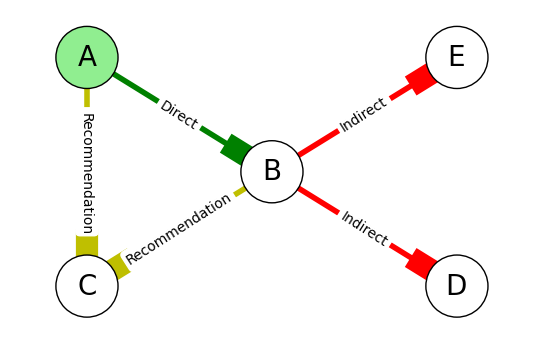
\includegraphics[width=.6\textwidth]{node_relationships}
      \label{fig:node_relationships}
    \end{figure}
    \footnotetext{\hyperlink{eq:networkeffects}{\beamergotobutton{Details}}}

\end{frame}

\begin{frame}{Multi-Metric Compared to Single in MANETs}
  Guo et al.\cite{Guo11} demonstrated that MTFM operates favourably in 802.11 based terrestrial MANETs against OTMF and Hermes, and can accurately detect, identify, \& characterise misbehaviours within a group of six nodes, with $n_0$ as the primary observer and $n_1$ as the misbehaver.

  \begin{figure}[h]
    \begin{center}
      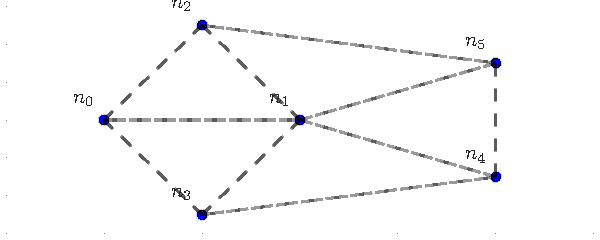
\includegraphics[width=0.6\textwidth]{s1_layout}
    \end{center}
    \caption{Initial Node Layouts in \cite{Guo11}}
    \label{fig:node_layout}
  \end{figure}
  \end{frame}

\subsection{Challenges to Trust in Underwater Networks}

\begin{frame}[allowframebreaks]{Communications Channel Considerations}
  Key Characteristics of the Marine Acoustic Channel \cite{Urick1983,Partan2006,Stojanovic2007,Stefanov2011}:
  \begin{itemize}
    \item Slow propagation ($~1400ms^{-1}$) incurring long delays
    \item Inter-symbol interference
    \item Doppler Spreading
    \item Non-Linear propagation due to refraction
    \item Fast \& Slow fades from environmental factors (flora/fauna/surface and seabed conditions)
    \item Freq. dependant attenuation
    \item Significant destructive multipath effects
  \end{itemize}
  
  \framebreak

  The attenuation that occurs in an underwater acoustic channel over a distance $d$ for a signal about frequency $f$ in linear power is given as $A_{\text{aco}}(d,f) = A_0d^ka(f)^d$ and in $dB$ form as;
  %
  \begin{equation}
    \label{eq:acoattenuationdb}
    10 \log A_{\text{aco}}(d,f)/A_0 = k \cdot 10 \log d + d \cdot 10 \log a(f)
  \end{equation}
  %
  where $A_0$ is a normalising constant, $k$ is a spreading factor (commonly taken as 1.5  \cite{Stojanovic2007}), and $a(f)$ is the absorption coefficient, approximated using Thorp's formula \cite{Stefanov2011}
  %
  \begin{equation}
    \label{eq:thorp}
    10 \log a(f) = \frac{0.11 \cdot f^2}{1+f^2} + \frac{44\cdot f^2}{4100+f^2}+ 2.75\times10^{-4} f^2 + 0.003
  \end{equation}

  \framebreak

  Compared to RF Free space PL: $(A_{\text{RF}}(d,f) \approx \left( \frac{4\pi d f}{c} \right)^2)$
  \begin{itemize}
    \item Exponential in $d$: $A_{\text{aco}} \propto f^{2d}$ vs $A_{\text{RF}} \propto (df)^2$
    \item Quadratic $f$ factor four orders higher in $f\propto A_{\text{aco}}$ vs $f\propto A_{\text{RF}}$

  \end{itemize}
  
\end{frame}




\section{Our Contribution}

\subsection{Experimental Context}
\begin{frame}{Operational Considerations: Collaborative AUV Survey}
  \begin{columns}
    \begin{column}{0.5\textwidth}
      Context:
      \begin{itemize}
        \item Fleets of up to 16 collaborating Autonomous Underwater Vehicles(AUVs)
        \item Constrained in Power, Mobility, Processing, Storage Capacity
        \item Tasked to perform ongoing survey of an area
      \end{itemize}

    Communications Efficiency is not the only operational asset at risk from malicious exploitation
      
    \end{column}
    \begin{column}{0.5\textwidth}
      \begin{figure}[h]
        \begin{center}
          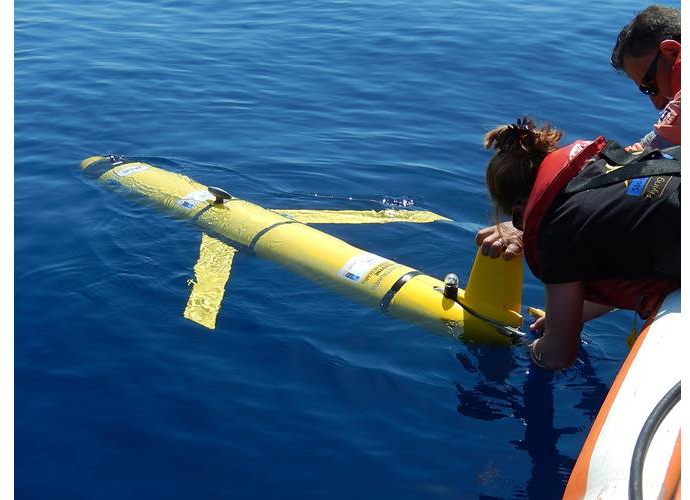
\includegraphics[width=\linewidth]{remus100cmre}
        \end{center}
        \caption{REMUS 100 AUV as deployed at NATO CMRE La Spezia}
        \label{fig:remus100cmre}
      \end{figure}
      
    \end{column}
  \end{columns}
\end{frame}

\begin{frame}{Scale Considerations}
  \begin{itemize}
    \item Simulations based on SimPy \cite{Mueller2003SimPy}, Network stack using AUVNetSim \cite{Miquel2008} and channel constraints based on Stojaovic and Stefanov \cite{Stojanovic2007,Stefanov2011}\hyperlink{tab:sysconstraints}{\beamergotobutton{Details}}
    \item Established a safe operating zone in terms of communications rate and node distances to optimise for delay/throughput at 0.015pps and avg. init. range 300m \hyperlink{eq:networkeffects}{\beamergotobutton{Details}}
    \item Six per-link communications metrics: TX/RX Throughput/Power, Delay and PLR, lacking the 802.11 Data Rate metric from \cite{Guo11}  
    
  \end{itemize}

\end{frame}

\begin{frame}{Misbehaviour Specification}
  Two misbehaviours developed:
  \begin{itemize}
    \item \emph{Malicious Power Control}(MPC) - attacker $n_1$ aims to make $n_0$ appear selfish by increasing power to all nodes except to/from $n_0$
    \item \emph{Selfish Target Selection}(STS) - $n_1$ preferentially communicates with nodes close to it, to conserve its own power.
  \end{itemize}

\end{frame}

\subsection{MTFM Operation}

\begin{frame}[allowframebreaks]{Multi-Metric Operation}
  \setcounter{subfigure}{0}% Reset subfigure counter
  \begin{figure}[htp]
    \centering
    \subfloat[Fair Static]{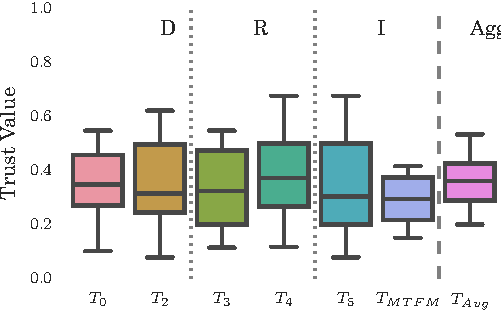
\includegraphics[width=0.33\linewidth]{trust_bella_static_fair} \label{fig:trust_static}}\hfil
    \subfloat[Malicious Static]{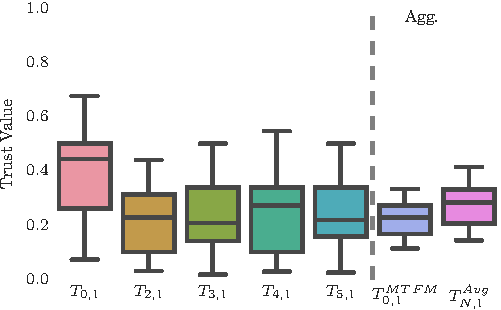
\includegraphics[width=0.33\linewidth]{trust_bella_static_malicious} \label{fig:trust_static_mal}}\hfil
    \subfloat[Selfish Static]{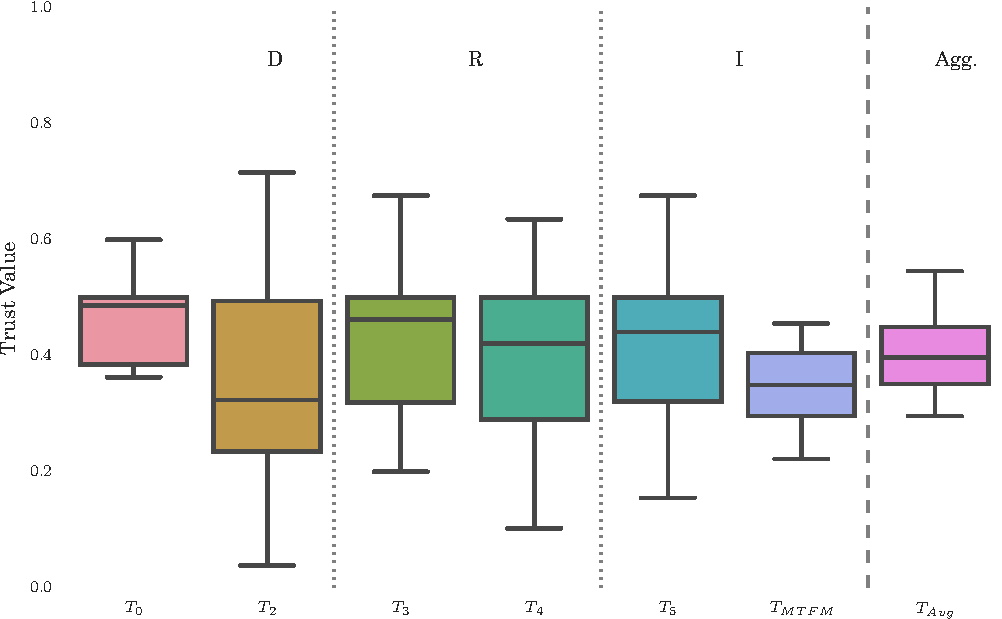
\includegraphics[width=0.33\linewidth]{trust_bella_static_selfish} \label{fig:trust_static_sel}}\hfil

    \subfloat[Fair Mobile]{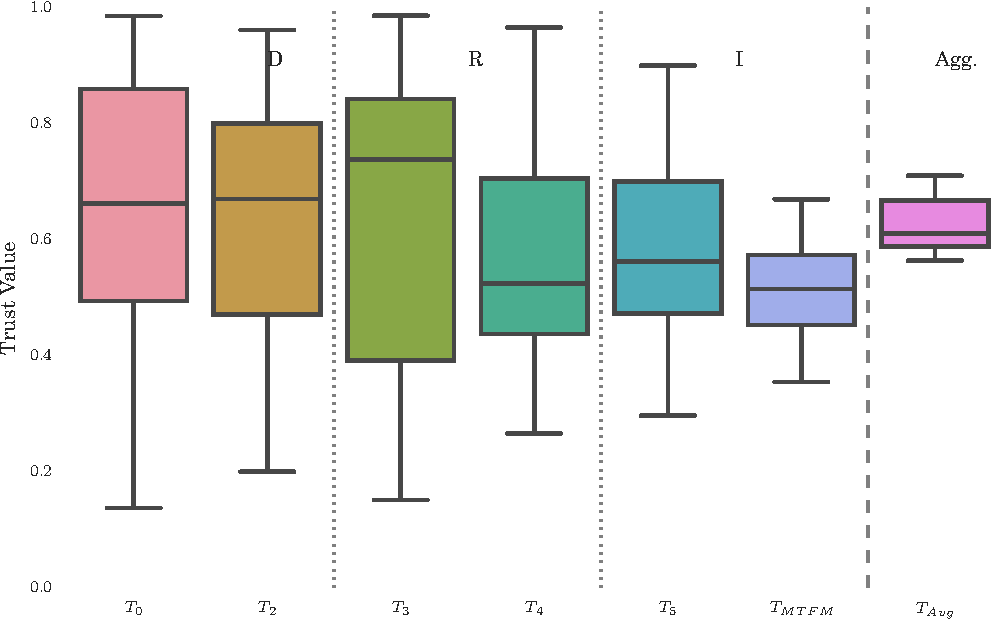
\includegraphics[width=0.33\linewidth]{trust_bella_all_mobile_fair}  \label{fig:trust_all_mobile}}\hfil
    \subfloat[Malicious Mobile]{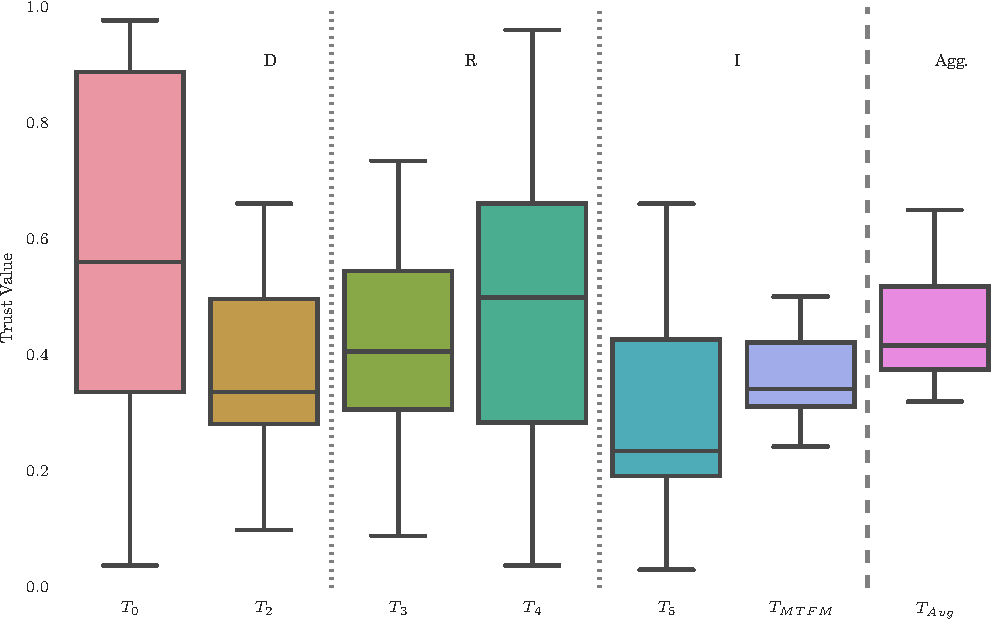
\includegraphics[width=0.33\linewidth]{trust_bella_all_mobile_malicious}  \label{fig:trust_all_mobile_mal}}\hfil
    \subfloat[Selfish Mobile]{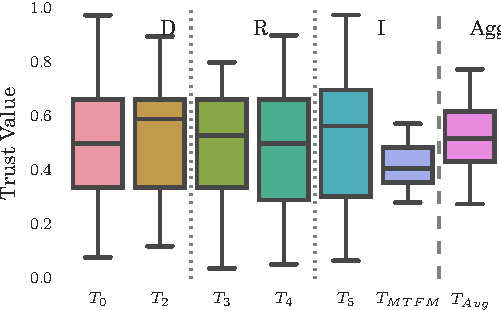
\includegraphics[width=0.33\linewidth]{trust_bella_all_mobile_selfish}  \label{fig:trust_all_mobile_sel}}\hfil
    \caption{Observations of $n_1$ ($T_{1,X}$), showing Direct, Recommender and Indirect relationships and $T_{MTFM}$ and $T_{AVG}$\hyperlink{fig:trust_mobility_closeup}{\beamergotobutton{Closeup}}}
    \label{fig:trust_mobility}
  \end{figure}
%\end{frame}
\framebreak
Key Observations: 
%\begin{frame}{Multi-Metric Operation - Key Observations}
  %
  \begin{itemize}
    \item Mobility greatly increases variation in instantaneously observed trust
    \item $T_{MTFM}$ remains more stable in both mobility cases when compared to either single-node assessments or $T_{Avg}$
    \item Raw $T_{MTGM}$ isn't perfect; in Fig~\ref{fig:trust_all_mobile_mal} demonstrates huge variability in Direct assessment ($T_{1,0}$) that isn't reflected in $T_{MTFM}$. Partially expected in this directed attack.
    \item Larger general variability in observations in ``Fair'' case compared to misbehaviours
  \end{itemize}
\end{frame}

\subsection{Single vs Multi}{Blind Comparison of Single/Multi-metric TMFs}

\begin{frame}[allowframebreaks,t]{Blind Comparison of Single/Multi-metric TMFs}
  \vspace{-24pt}%
  \begin{columns}
    \begin{column}[T]{0.5\textwidth}
      \begin{figure}[t]
        \centering
        \subfloat[Fair Scenario]{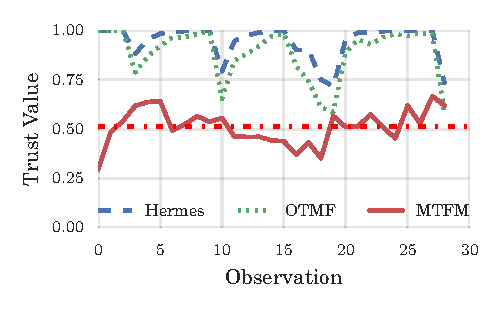
\includegraphics[width=\linewidth]{trust_beta_otmf_fair} \label{fig:all_mobile_fair_beta}}\hfil
        \renewcommand{\thesubfigure}{c}% New fixed/manual numbering
        \subfloat[Selfish Target Selection Scenario]{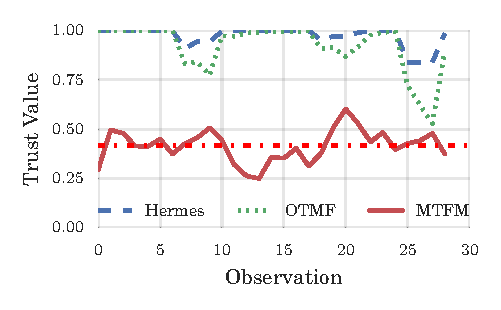
\includegraphics[width=\linewidth]{trust_beta_otmf_selfish} \label{fig:all_mobile_selfish_beta}}
        \label{fig:otmf_beta_comparison}
      \end{figure}%
    \end{column}
    \begin{column}[T]{0.5\textwidth}
      \begin{figure}[t]
        \centering
        \vspace{0pt}%
        \renewcommand{\thesubfigure}{b}% New fixed/manual numbering
        \subfloat[Malicious Power Control Scenario]{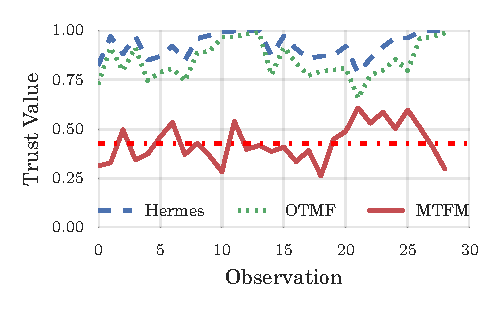
\includegraphics[width=\linewidth]{trust_beta_otmf_malicious} \label{fig:all_mobile_badmouthing_beta}}
        \label{fig:otmf_beta_comparison}
      \end{figure}
      $T_{1,0}$ for Hermes, OTMF and MTFM assessment values for fair and malicious behaviours in the fully mobile scenario (mean of MTFM also shown)

    \end{column}
  \end{columns}

  \framebreak

  Key Observations:
  \begin{itemize}
    \item Neither misbehaviour, while impacting network fairness, directly affects PLR
    \item MTFM's Cohort Comparison means in the fair case, 0.5 is expected
    \item In OTMF/Hermes, $T~1$ is expected
    \item Neither OTMF, Hermes or Blind MTFM are particularly effective
    \item MTFM indicates $~10\%$ selectivity between Fair and Either Misbehaviour
  \end{itemize}

\end{frame}

\subsection{Metric Weighting}
\begin{frame}{Metric Weighting}
  From \ref{eq:grc}, metric emphasise can be adjusted, highlighting misbehaviour in particular metric areas
  \begin{align}
    [\theta_k^t, \phi_k^t]& = \left[\sum_{j=0}^M h_j \theta_{k,j}^t,\sum_{j=0}^M h_j \phi_{k,j}^t \right]\\
    T_k^t &= ({1+{(\phi_k^t)^2}/{(\theta_k^t)^2}})^{-1}
    \label{<++>}
  \end{align}
\end{frame}

\begin{frame}{Malicious Power Control - Weighted Emphasis}
  \vspace{-24pt}%
\setcounter{subfigure}{0}% Reset subfigure counter
  \begin{figure}[h]
    \centering
    \subfloat[Delay Emphasised]{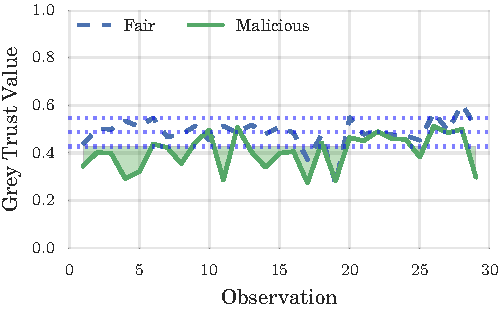
\includegraphics[width=.33\linewidth]{img/trust_bella_all_mobile_emph_ADelay_BadMouthingPowerControl} \label{fig:all_mobile_badmouthing_delay}}
    \subfloat[PLR Emphasised]{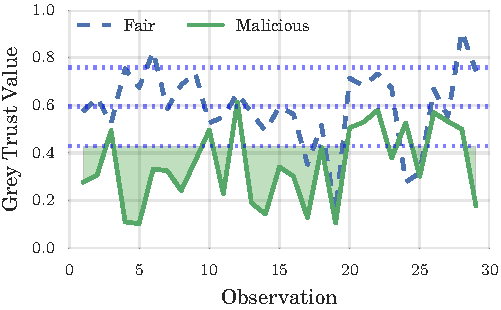
\includegraphics[width=.33\linewidth]{img/trust_bella_all_mobile_emph_PLR_BadMouthingPowerControl}\label{fig:all_mobile_badmouthing_plr}}
    \subfloat[RX Power Emphasised]{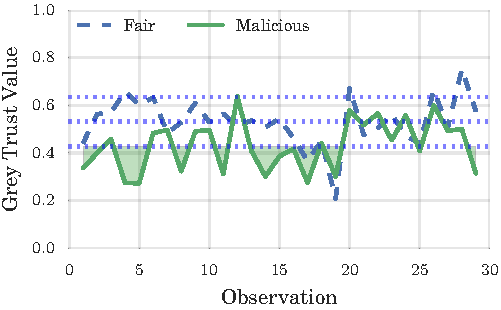
\includegraphics[width=.33\linewidth]{img/trust_bella_all_mobile_emph_ARXP_BadMouthingPowerControl} \label{fig:all_mobile_badmouthing_rxp}}
    \newline
    \subfloat[TX Power Emphasised]{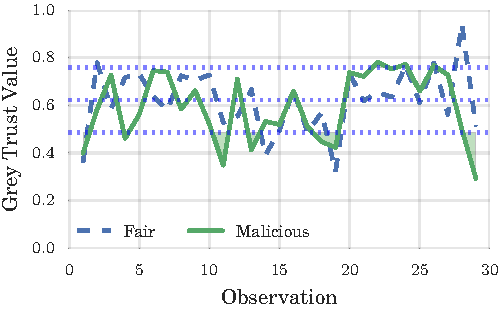
\includegraphics[width=.33\linewidth]{img/trust_bella_all_mobile_emph_ATXP_BadMouthingPowerControl}\label{fig:all_mobile_badmouthing_txp}}
    \subfloat[RX Throughput Emphasised]{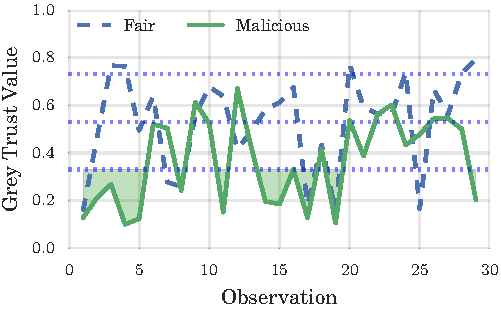
\includegraphics[width=.33\linewidth]{img/trust_bella_all_mobile_emph_RXThroughput_BadMouthingPowerControl} \label{fig:all_mobile_badmouthing_rxthroughput}}
    \subfloat[TX Throughput Emphasised]{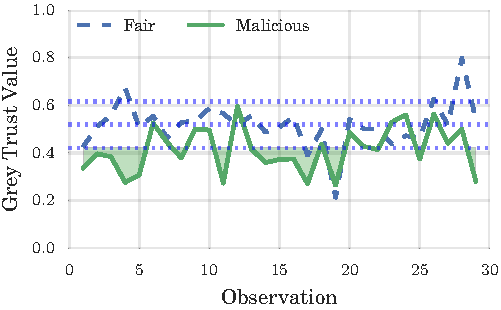
\includegraphics[width=.33\linewidth]{img/trust_bella_all_mobile_emph_TXThroughput_BadMouthingPowerControl} \label{fig:all_mobile_badmouthing_txthroughput}}
    \caption{$T_{1,MTFM}$ in the All Mobile case for the Malicious Power Control behaviour, including dashed $\pm\sigma$ envelope about the fair scenario\hyperlink{fig:badmouth_emph_closeup}{\beamergotobutton{Closeup}}}
    \label{fig:all_mobile_badmouthing}
  \end{figure}
\end{frame}

\begin{frame}{Selfish Target Selection - Weighted Emphasis}
  \vspace{-24pt}%
\setcounter{subfigure}{0}% Reset subfigure counter
  \begin{figure}[h]
  \centering
  \subfloat[Delay Emphasised]{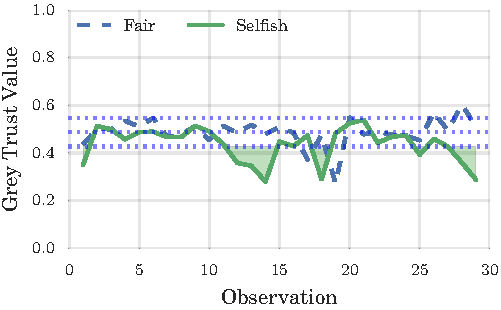
\includegraphics[width=.33\linewidth]{img/trust_bella_all_mobile_emph_ADelay_SelfishTargetSelection} \label{fig:all_mobile_selfish_delay}}
  \subfloat[PLR Emphasised]{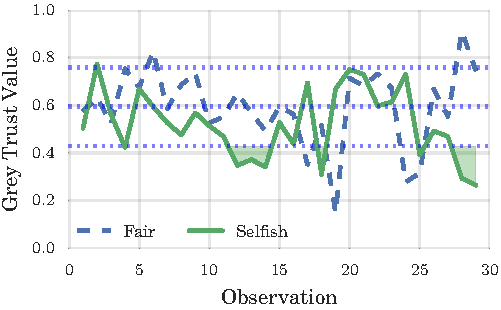
\includegraphics[width=.33\linewidth]{img/trust_bella_all_mobile_emph_PLR_SelfishTargetSelection}\label{fig:all_mobile_selfish_plr}}
  \subfloat[RX Power Emphasised]{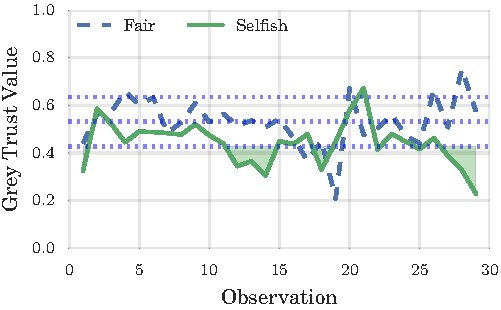
\includegraphics[width=.33\linewidth]{img/trust_bella_all_mobile_emph_ARXP_SelfishTargetSelection} \label{fig:all_mobile_selfish_rxp}}
  \newline
  \subfloat[TX Power Emphasised]{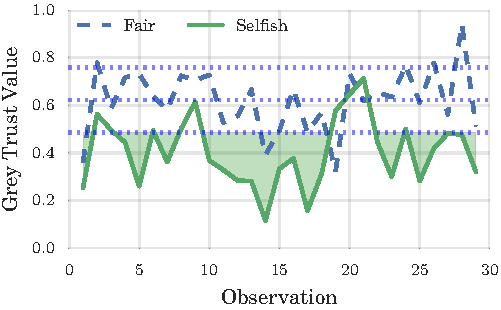
\includegraphics[width=.33\linewidth]{img/trust_bella_all_mobile_emph_ATXP_SelfishTargetSelection}\label{fig:all_mobile_selfish_txp}}
  \subfloat[RX Throughput Emphasised]{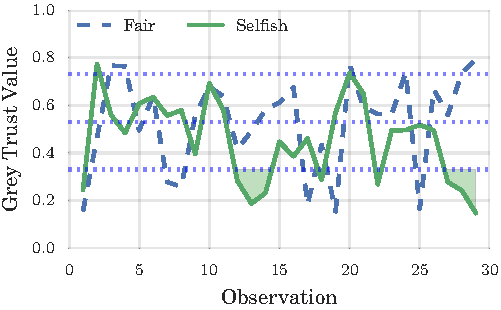
\includegraphics[width=.33\linewidth]{img/trust_bella_all_mobile_emph_RXThroughput_SelfishTargetSelection} \label{fig:all_mobile_selfish_rxthroughput}}
  \subfloat[TX Throughput Emphasised]{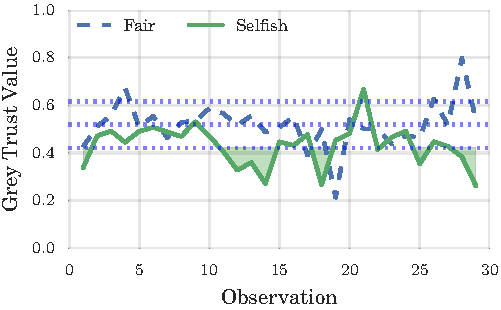
\includegraphics[width=.33\linewidth]{img/trust_bella_all_mobile_emph_TXThroughput_SelfishTargetSelection} \label{fig:all_mobile_selfish_txthroughput}}
\caption{$T_{1,MTFM}$ in the All Mobile case for the Selfish Target Selection behaviour, including dashed $\pm\sigma$ envelope about the fair scenario\hyperlink{fig:selfish_emph_closeup}{\beamergotobutton{Closeup}}}
 
\label{fig:all_mobile_selfish}
\end{figure}
\end{frame}

\begin{frame}{Metric Weighting}
  Key Observations:
  \begin{itemize}
    \item In MPC case:
      \begin{itemize}
        \item Consistently outside $\pm\sigma$ in all but $P_{TX}$, particularly PLR
        \item Less so in Delay, $P_{RX}$ and $T_{TX}$
      \end{itemize}
    \item In STS case:
      \begin{itemize}
        \item Less overall impact, except when $P_{TX}$
      \end{itemize}

    \item In General:
      \begin{itemize}
        \item Qualatatively similar to similar experiments performed in \cite{Guo11} in RF Terrestrial MANET
        \item Lower differences between misbehaviour/fair cases
        \item Less consistent deviations
        \item More useful than OTMF/Hermes but still not perfect
      \end{itemize}
  \end{itemize}

\end{frame}


\subsection{Metric Significance}
\begin{frame}[allowframebreaks]{Regression of Metric Significance}
  \begin{itemize}
    \item Distributed Random Forest Regression \cite{Breiman2001} 
    \item 729 Metric Weight Vectors ($H$), 512 random trees
    \item 16 Random starts of each of the 3 scenarios for 6 nodes for 6 hour ``missions''
    \item Targeting area of $\pm\sigma$ deviation $\int abs(T_m - \overline T_f) - \sigma_{T_f}$
    \item Regression identifies the significance of metrics in classifying between the three possible behaviours
  \end{itemize}

  \framebreak

  \begin{figure}
    \centering
    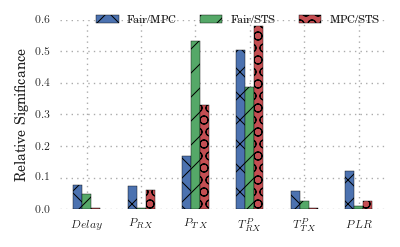
\includegraphics[width=0.95\linewidth]{img/MaliciousSelfishMetricFactors}
    \label{fig:malselfactors}
  \end{figure}
  \vspace{-30pt}%
  \begin{table}[h]
    \begin{center}
      \small
      \bgroup
      \def\arraystretch{1.2}%  1 is the default, change whatever you need
      \setlength\tabcolsep{4pt}% 6pt standard
      \begin{tabular}{l|CCCCCC}
        \toprule
        Correlation      & Delay & $P_{RX}$ & $P_{TX}$ & $T^P_{RX}$ & $T^P_{TX}$ & PLR \\
        \midrule
        Fair / MPC       & 0.199 &  0.159   & -0.416  &  0.708   & -0.238   & -0.401\\
        Fair / STS       & 0.179 &  -0.009  &  0.724  & -0.697   & -0.145   & -0.052\\
        MPC / STS        & 0.058 &  -0.134  &  0.146  & -0.768   &  0.052   &  0.146\\
        \bottomrule
      \end{tabular}
      \egroup
    \end{center}
  \end{table}

  \framebreak

  Key Observations:
  \begin{itemize}
    \item PLR not necessarily the most important metric
    \item Combination of Significance and Correlations demonstrate selectivity opportunity
    \item MTFM has capability to finely discriminate between similar misbehaviours
    \item PLR impact is minimal in STS, would not be detected by OTMF/Hermes even in less sparse/harsh environment
    \item Identifying this classification ``comb'' is computationally intensive and grows exponentially with number of metrics involved for brute force regression
  \end{itemize}
\end{frame}

\subsection{Current Work}

\begin{frame}{Current Work and Paths to Proof/Implementation}
  \begin{itemize}
    \item Include Physical Observations in Metric Set
      \begin{itemize}
        \item Assess benefits / drawbacks of domain separation / joining
        \item Assess complexity vs selectivity of derived classifications
      \end{itemize}
    \item Perform / Initiate practical trials in collaborations with NATO CMRE
  \end{itemize}
\end{frame}



\section*{Summary}

\begin{frame}{Summary}

  % Keep the summary *very short*.
  \begin{itemize}
    \item Trust Underwater is \alert{Hard}, but it's mostly the environments' fault
    \item Single-Metric Trust is \alert{unstable} in such an environment
    \item Multi-Metric Trust works and can \alert{discriminate between behaviours}
    \item \alert{Not all metrics} are equally useful
  \end{itemize}
  
  % The following outlook is optional.
  \vskip0pt plus.5fill
  \begin{itemize}
  \item
    Outlook
    \begin{itemize}
    \item
      Extending to include Physical Metrics
    \item
      Developing runtime heuristics to improve complexity
    \item 
      Perform untrained classification performance on real data      
    \end{itemize}
  \end{itemize}
\end{frame}

\begin{frame}[t,allowframebreaks]
  \frametitle{References}
  \printbibliography[title=References]% [nottype=video]}
\end{frame}

\begin{frame}
  \centerline{The End}
\end{frame}

\begin{frame}[allowframebreaks]{Grey Trust Equs}
\todo{Add backlinks}
  \begin{align}
    \label{eq:networkeffects}
    T_{i,j}^{MTFM}=&\frac{1}{2} \cdot \max_s\{f_s(T_{i,j})\} T_{i,j}\\ \notag
    +&\frac{1}{2} \frac{2|N_R| }{2|N_R| + |N_I|}\sum_{n \in N_R} \max_s\{f_s(T_{i,n})\} T_{i,n}\\ \notag
    +&\frac{1}{2} \frac{|N_I| }{2|N_R| + |N_I|}\sum_{n \in N_I} \max_s\{f_s(T_{i,n})\} T_{i,n} 
  \end{align}

  Where $T_{i,n}$ is the subjective trust assessment of $n_i$ by $n_n$, and $f_s = [ f_1,f_2, f_3]$ given as...

  \framebreak

  \begin{align}
    \label{eq:whitenization}
    f_1(x)&= -x+1\notag\\
    f_2(x)&= 
    \begin{cases}
      2x & \text{if }x\leq 0.5\\
      -2x+2 & \text{if }x>0.5
    \end{cases}\\
    f_3(x)&= x\notag
  \end{align}
\end{frame}

\begin{frame}[allowframebreaks]{Comms Scaling Graphs}

\setcounter{subfigure}{0}% Reset subfigure counter
  \begin{figure}[h]
    \centering
    \subfloat[][All Nodes Static]{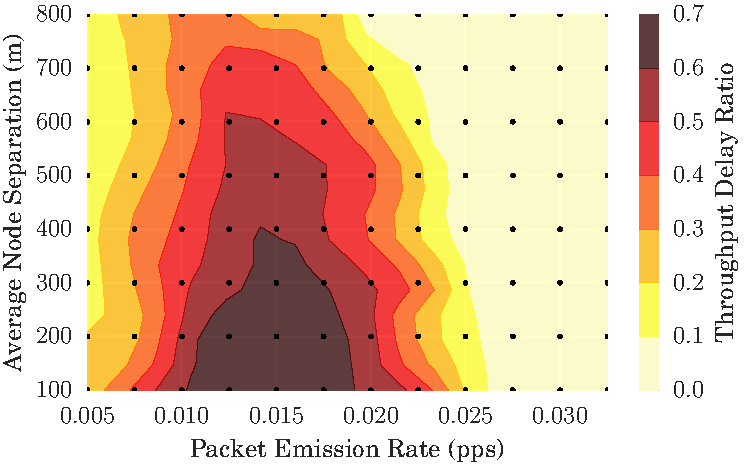
\includegraphics[width=0.35\linewidth]{2d_ratio_static.pdf}}
    \subfloat[][$n_1$ Random Walk]{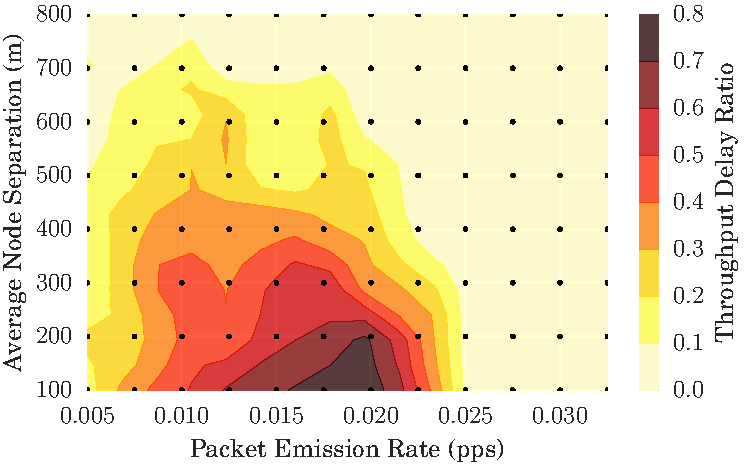
\includegraphics[width=0.35\linewidth]{2d_ratio_single_mobile.pdf}}\\
    \subfloat[][All nodes but $n_1$ Random Walk]{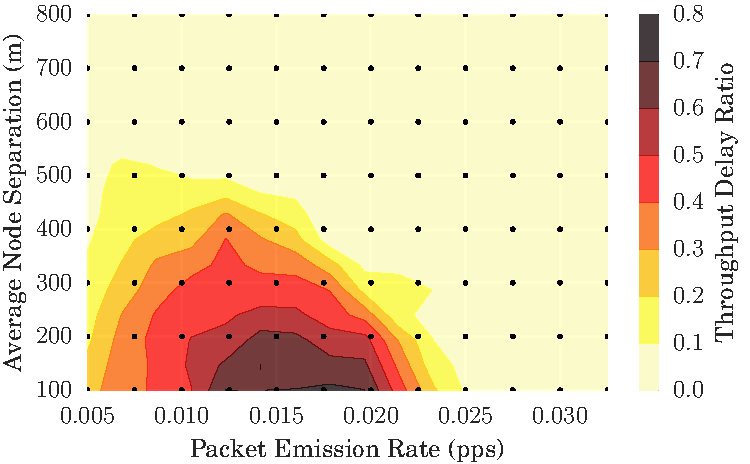
\includegraphics[width=0.35\linewidth]{2d_ratio_allbut1.pdf}}
    \subfloat[][All nodes Random Walk]{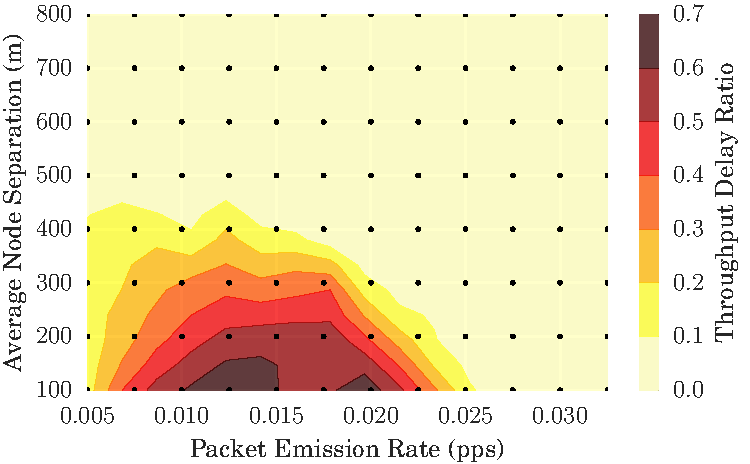
\includegraphics[width=0.35\linewidth]{2d_ratio_all_mobile.pdf}}
    \label{fig:CommsThroughputRatios}
  \end{figure}

\end{frame}

\begin{frame}[shrink]{System Model Constraints}
\centering
\begin{table}[h]
  \caption{Comparison of system model constraints as applied between Terrestrial and Marine communications} \label{tab:sysconstraints}
  \begin{center}
    \setlength{\tabcolsep}{8pt}
    \begin{tabular}{lccc}
      \toprule
      Parameter & Unit & Terrestrial & Marine \\
      \midrule
      Simulated Duration & $s$ & 300 & 18000\\
      Trust Sampling Period & $s$ & 1 & 600 \\
      Simulated Area & $km^2$ & 0.7 & 0.7-4 \\
      Transmission Range & $km$ & 0.25 & 1.5 \\
      Physical Layer & & RF(802.11) & Acoustic\\
      Propagation Speed& $m/s$ & $3\times10^8$ & 1490\\
      Center Frequency& $Hz$ & $2.6\times10^9$ & $2 \times 10^4$ \\
      Bandwidth& $Hz$ & $22\times10^6$ & $1\times10^4$\\
      MAC Type & & CSMA/DCF & CSMA/CA\\
      Routing Protocol & & DSDV & FBR \\
      Max Speed & $ms^{-1}$ & 5 & 1.5 \\
      Max Data Rate & $bps$ & $5\times10^6$ & $\approx 240$ \\
      Packet Size & bits & 4096 &  9600 \\
      Single Transmission Duration & $s$ & 10 & 32 \\
      Single Transmission Size & bits & $10^7$ & $9600$ \\
      \bottomrule
    \end{tabular}
    \setlength{\tabcolsep}{6pt}
  \end{center}
\end{table}

\end{frame}

\begin{frame}{MTFM Operation Detail}
%
\setcounter{subfigure}{0}% Reset subfigure counter
\label{fig:trust_mobility_closeup}%
\begin{figure}[h]
  \subfloat[Fair Static]{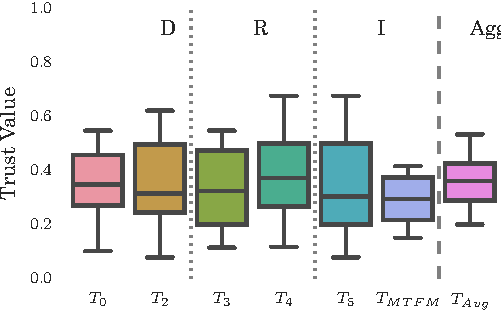
\includegraphics[width=1.0\linewidth]{trust_bella_static_fair} \label{fig:trust_static}}
\end{figure}
\todo{Add backlinks}
\end{frame}
\begin{frame}{MTFM Operation Detail}
\begin{figure}[h]
  \subfloat[Malicious Static]{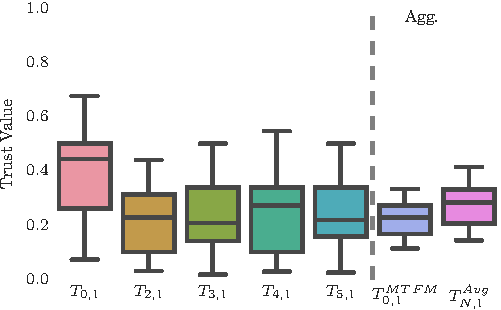
\includegraphics[width=1.0\linewidth]{trust_bella_static_malicious} \label{fig:trust_static_mal}}
\end{figure}
\end{frame}
\begin{frame}{MTFM Operation Detail}
\begin{figure}[h]
  \subfloat[Selfish Static]{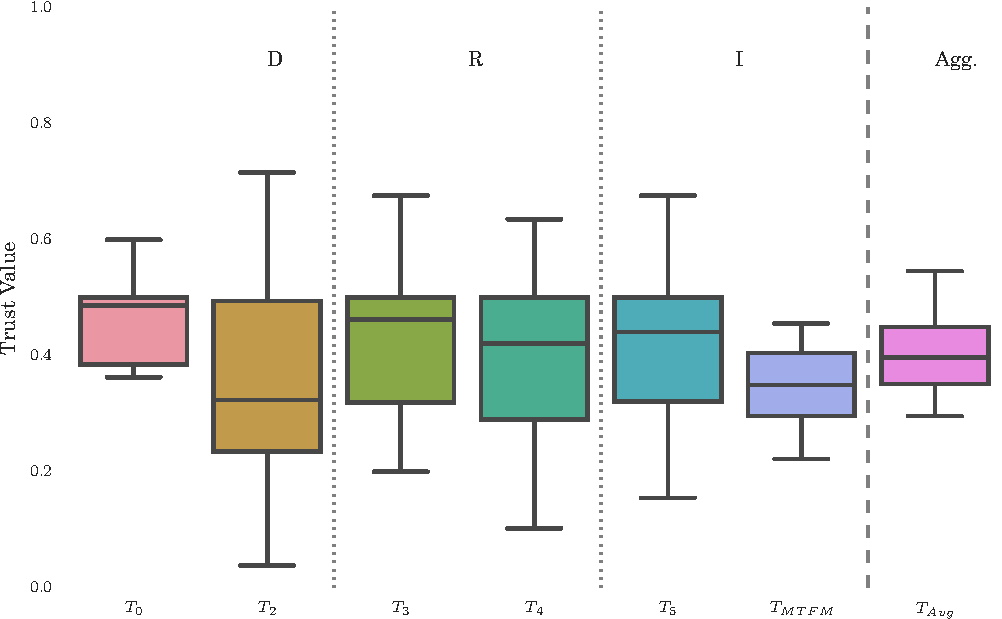
\includegraphics[width=1.0\linewidth]{trust_bella_static_selfish} \label{fig:trust_static_sel}}
\end{figure}
\end{frame}
\begin{frame}{MTFM Operation Detail}
\begin{figure}[h]
  \subfloat[Fair Mobile]{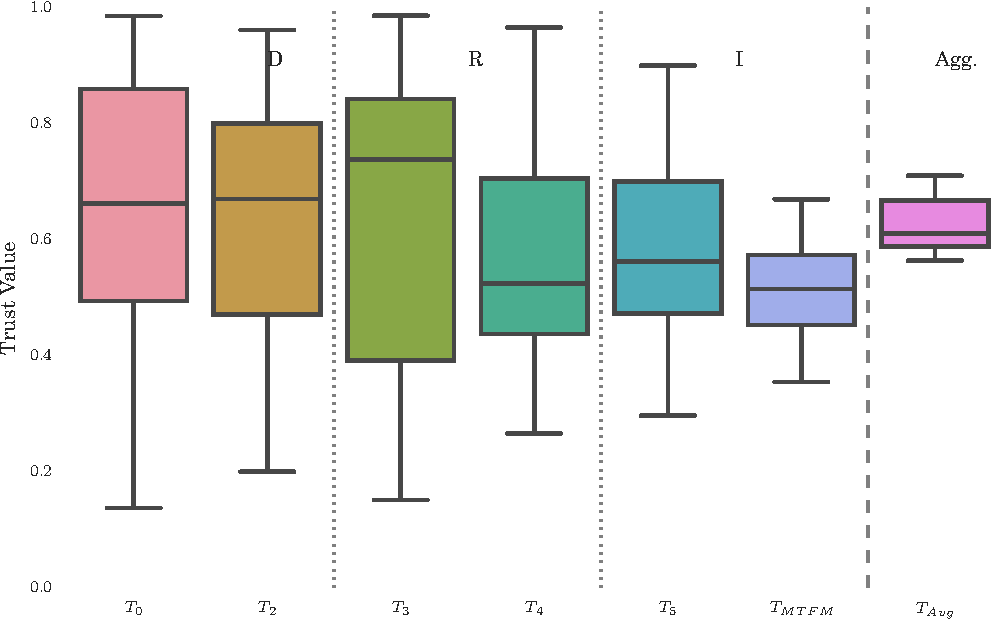
\includegraphics[width=1.0\linewidth]{trust_bella_all_mobile_fair}  \label{fig:trust_all_mobile}}
\end{figure}
\end{frame}
\begin{frame}{MTFM Operation Detail}
\begin{figure}[h]
  \subfloat[Malicious Mobile]{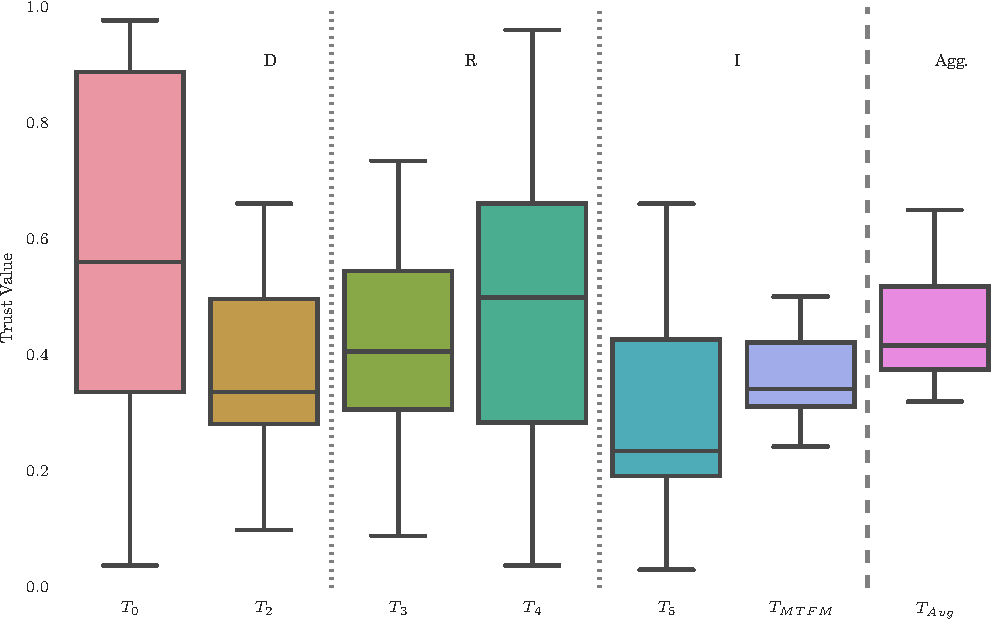
\includegraphics[width=1.0\linewidth]{trust_bella_all_mobile_malicious}  \label{fig:trust_all_mobile_mal}}
\end{figure}
\end{frame}
\begin{frame}{MTFM Operation Detail}
\begin{figure}[h]
  \subfloat[Selfish Mobile]{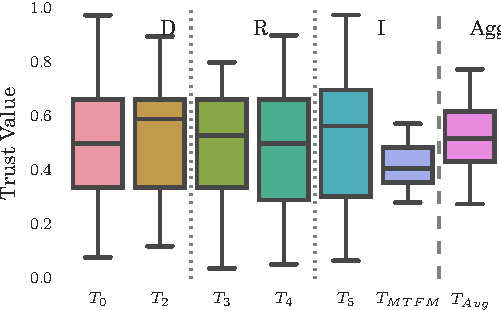
\includegraphics[width=1.0\linewidth]{trust_bella_all_mobile_selfish}  \label{fig:trust_all_mobile_sel}}
\end{figure}
\end{frame}


\begin{frame}{MTFM Malicious Power Control Detail}
\setcounter{subfigure}{0}% Reset subfigure counter
\label{fig:badmouth_emph_closeup}%
\begin{figure}[h]
  \subfloat[Delay Emphasised]{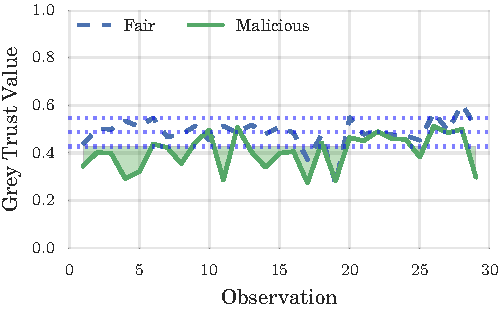
\includegraphics[width=\linewidth]{img/trust_bella_all_mobile_emph_ADelay_BadMouthingPowerControl} \label{fig:all_mobile_badmouthing_delay}}
\end{figure}
\todo{Add backlinks}
\end{frame}
\begin{frame}{MTFM Malicious Power Control Detail}
\begin{figure}[h]
  \subfloat[PLR Emphasised]{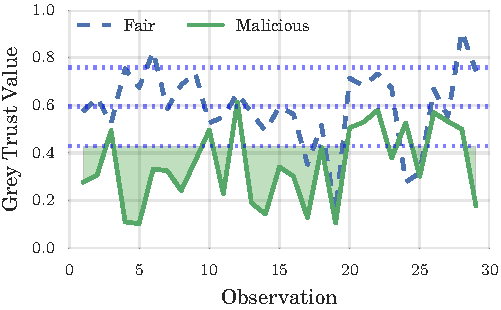
\includegraphics[width=\linewidth]{img/trust_bella_all_mobile_emph_PLR_BadMouthingPowerControl}\label{fig:all_mobile_badmouthing_plr}}
\end{figure}
\end{frame}
\begin{frame}{MTFM Malicious Power Control Detail}
\begin{figure}[h]
  \subfloat[RX Power Emphasised]{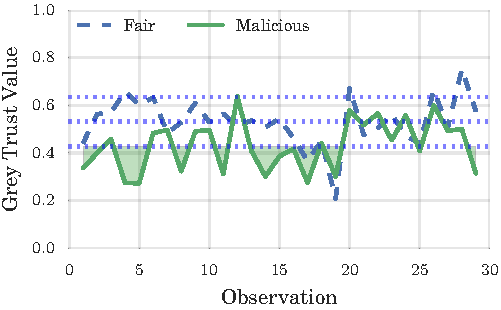
\includegraphics[width=\linewidth]{img/trust_bella_all_mobile_emph_ARXP_BadMouthingPowerControl} \label{fig:all_mobile_badmouthing_rxp}}
\end{figure}
\end{frame}
\begin{frame}{MTFM Malicious Power Control Detail}
\begin{figure}[h]
  \subfloat[TX Power Emphasised]{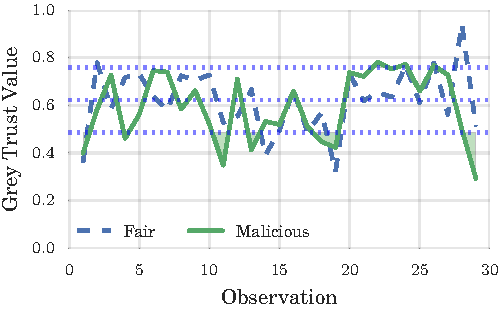
\includegraphics[width=\linewidth]{img/trust_bella_all_mobile_emph_ATXP_BadMouthingPowerControl}\label{fig:all_mobile_badmouthing_txp}}
\end{figure}
\end{frame}
\begin{frame}{MTFM Malicious Power Control Detail}
\begin{figure}[h]
  \subfloat[RX Throughput Emphasised]{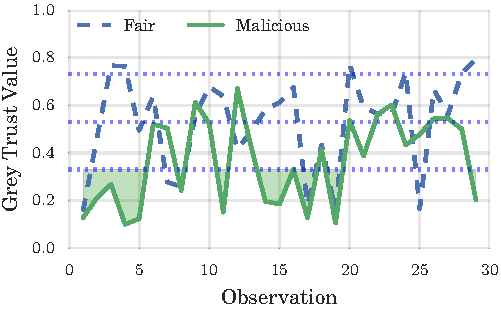
\includegraphics[width=\linewidth]{img/trust_bella_all_mobile_emph_RXThroughput_BadMouthingPowerControl} \label{fig:all_mobile_badmouthing_rxthroughput}}
\end{figure}
\end{frame}
\begin{frame}{MTFM Malicious Power Control Detail}
\begin{figure}[h]
  \subfloat[TX Throughput Emphasised]{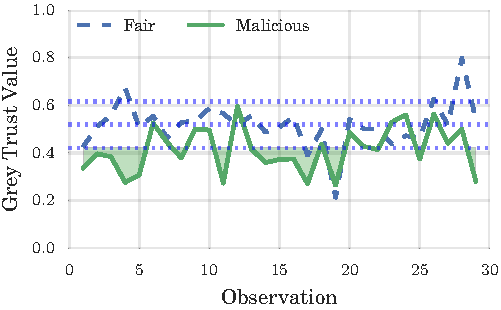
\includegraphics[width=\linewidth]{img/trust_bella_all_mobile_emph_TXThroughput_BadMouthingPowerControl} \label{fig:all_mobile_badmouthing_txthroughput}}
\end{figure}
\end{frame}
\begin{frame}{MTFM Selfish Target Selection Detail}
\setcounter{subfigure}{0}% Reset subfigure counter
\label{fig:selfish_emph_closeup}%
\begin{figure}[h]
  \subfloat[Delay Emphasised]{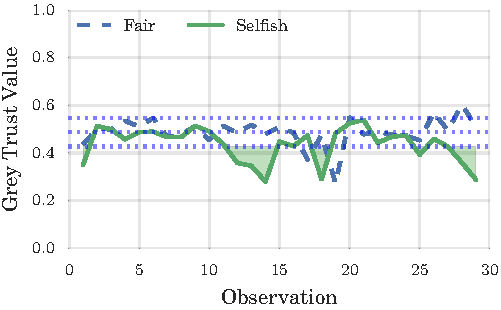
\includegraphics[width=\linewidth]{img/trust_bella_all_mobile_emph_ADelay_SelfishTargetSelection} \label{fig:all_mobile_selfish_delay}}
\end{figure}
\todo{Add backlinks}
\end{frame}
\begin{frame}{MTFM Selfish Target Selection Detail}
\begin{figure}[h]
  \subfloat[PLR Emphasised]{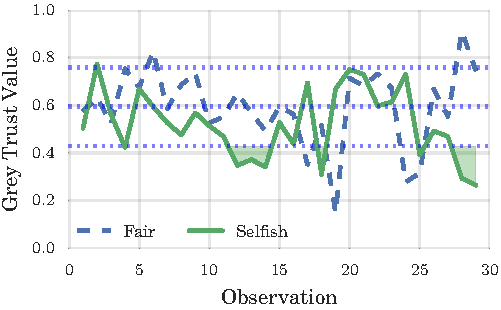
\includegraphics[width=\linewidth]{img/trust_bella_all_mobile_emph_PLR_SelfishTargetSelection}\label{fig:all_mobile_selfish_plr}}
\end{figure}
\end{frame}
\begin{frame}{MTFM Selfish Target Selection Detail}
\begin{figure}[h]
  \subfloat[RX Power Emphasised]{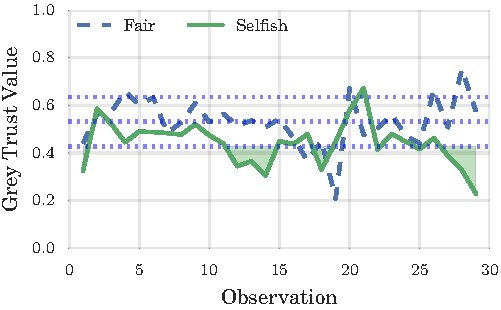
\includegraphics[width=\linewidth]{img/trust_bella_all_mobile_emph_ARXP_SelfishTargetSelection} \label{fig:all_mobile_selfish_rxp}}
\end{figure}
\end{frame}
\begin{frame}{MTFM Selfish Target Selection Detail}
\begin{figure}[h]
  \subfloat[TX Power Emphasised]{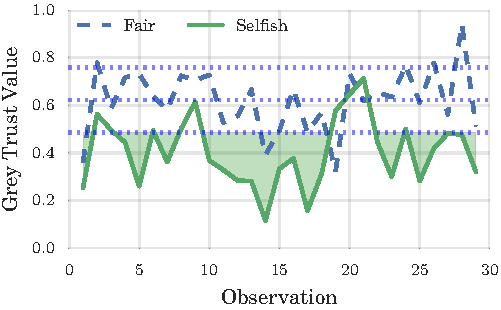
\includegraphics[width=\linewidth]{img/trust_bella_all_mobile_emph_ATXP_SelfishTargetSelection}\label{fig:all_mobile_selfish_txp}}
\end{figure}
\end{frame}
\begin{frame}{MTFM Selfish Target Selection Detail}
\begin{figure}[h]
  \subfloat[RX Throughput Emphasised]{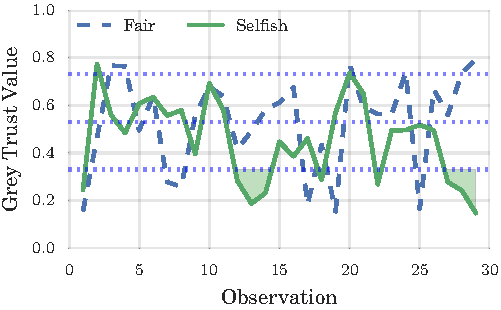
\includegraphics[width=\linewidth]{img/trust_bella_all_mobile_emph_RXThroughput_SelfishTargetSelection} \label{fig:all_mobile_selfish_rxthroughput}}
\end{figure}
\end{frame}
\begin{frame}{MTFM Selfish Target Selection Detail}
\begin{figure}[h]
  \subfloat[TX Throughput Emphasised]{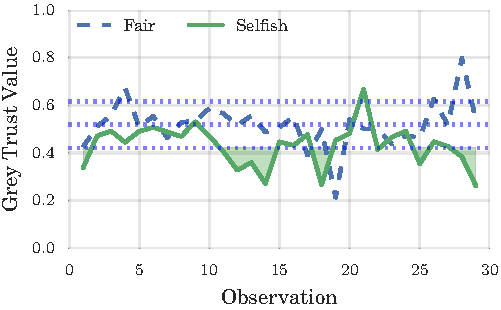
\includegraphics[width=\linewidth]{img/trust_bella_all_mobile_emph_TXThroughput_SelfishTargetSelection} \label{fig:all_mobile_selfish_txthroughput}}
\end{figure}
\end{frame}

\end{document}
